\chapter{Ideal Gas and Thermal Conductivity}
\label{chap:gas}
\section{Introduction}

Thermodynamics is critical in presiding over how the universe functions.  From explaining how molecular bonds in a liquid break as the particles become gaseous, to explaining the disappearance or ``evaporation" of black holes, thermodynamics is instrumental in the dominion of the microscopic through macroscopic.  Over the course of the Earth's history evolution began and has proceeded by reacting to and occasionally altering the world's temperature - accustoming itself to the continuity of general thermal equilibrium, while adapting to minor and major fluctuations that occur over periods of days days to millions of years.  Though typically overlooked, thermodynamics is essential in our interactions with the world and the decisions we make on a near-constant basis: from dressing warmly to combat the cold air, to popping our ears upon changing altitudes, to constructing buildings that insulate us from weather.\myskip

The purpose of this lab is to study three significant consequences of thermodynamics.  Specifically, we want to:
\begin{enumerate}
\item verify the ideal gas law,
\item understand thermal conductivity and how it varies in different materials, and
\item observe and comprehend certain simple thermal processes and their effects on an ideal gas.
\end{enumerate}

\section{Theory}
\label{thermtheory}
\subsection{Ideal Gas Law}
\label{idealtheory}
The ideal gas law is the equation of state for a gas of particles (typically atoms or molecules) under ``normal" lab settings (i.e. temperature is sufficiently high to negate weakly attractive forces between molecules, and the volume of the gas is relatively large compared to that of the particles).  It reads

\begin{equation}
\label{eq:ideal}
PV=NkT
\end{equation}

\noindent where $P$ is the pressure of the gas, $V$ is the volume it occupies, $N$ is the number of particles, $k$ is Boltzmann's constant ($1.38 \cdot 10^{-23}$ J/K), and $T$ is the temperature (in Kelvin).  You may also have seen this written as $PV=nRT$ where $n \equiv N/N_{\rm A}$ is the number of moles, and $R \equiv kN_{\rm A}$ is known as the gas constant ($N_{\rm A} = 6.02 \cdot 10^{23}$ particles/mole is Avogadro's Number).  You can use either form of the ideal gas law in this experiment.\myskip

For the experiments in Sections \ref{procideal} and \ref{procadiab} we will be manipulating gases by changing their volumes while keeping the number of particles $N$ constant.  In the Section \ref{procideal} we will monitor $P$ and $T$ as our container suddenly shifts from $V_{1}$ to $V_{2}$.  To understand how our gas reacts, we need to use the First Law of Thermodynamics

\begin{equation}
\label{eq:firstlaw}
\Delta E = Q - W
\end{equation}

\noindent where  $\Delta E$ is the internal energy of the gas, $Q$ is any heat added, and $W$ is the work the substance does by expanding in volume.  Think of the First Law as conservation of energy, stating that any added (or subtracted) heat must equal the change in energy of the gas plus the work that gas does on its surroundings.\myskip

In general we must consider Equation \ref{eq:firstlaw} to evaluate how Equation \ref{eq:ideal} changes under various thermodynamic processes.  This can often be complicated, as even with a gas of fixed $N$ particles, $P$, $V$, and $T$ are all subject to change.  However, we are often interested in processes that leave one of these variables fixed, as seen in Table \ref{processes}.  For this lab we are going to mainly consider \textit{isochoric} and \textit{adiabatic} processes.\myskip

\begin{table}
\begin{center}
\begin{tabular}{| c | c | c | c |}
\hline
	Constraints & Name & First Law Simplified & Ideal Gas Law Simplified \\
	\hline
	$P$ = Constant & Isobaric & $\Delta E = Q - W$ & $V \propto T$ \\
	$V$ = Constant & Isochoric & $\Delta E = Q$ & $P \propto T$ \\
	$T$ = Constant & Isothermal & $0 = Q - W$ & $P \propto V^{-1}$ \\
	$Q = 0$ & Adiabatic & $\Delta E = W$ & $PV \propto T$ \\
	\hline
\end{tabular}
\end{center}
\caption{Thermodynamic constraints that permit simplifications in the ideal gas law and the First Law of Thermodynamics.}
\label{processes}
\end{table}

In the case of a sudden or instantaneous change in volume, there is no time for heat to be exchanged between a gas and its encompassing environment, so $Q=0$.  This is known as an \textit{adiabatic compression/expansion}.  Experiments in both Sections \ref{procideal} and \ref{procadiab} will involve compressions, allowing us to quantitatively and qualitatively, respectively, observe the effects.  Because no heat is allowed to escape, adiabatic compression is typically the fastest way to increase the thermal energy of the gas.  In Section \ref{procadiab} we will demonstrate this effect to light a piece of paper on fire by suddenly compressing a small volume of air.\myskip

It is also useful to understand \textit{isochoric processes}: how heat is exchanged between a gas at constant volume and its surroundings.  This concept is likely very familiar in your own life: two (not necessarily different) materials at different temperatures that are in contact with each other will attempt to attain thermal equilibrium - that is, they will exchange heat until they both have the same temperature.  In this lab we will demonstrate that after a gas in a chamber is heated up and then kept at constant volume, its temperature will slowly decline due to thermal exchanges with the surrounding air in the room.\myskip

\subsection{Thermal Conductivity}
The end of the previous section might instill a desire to understand how materials at different temperatures equilibrate when they cannot directly interact with each other, but instead have a medium between them.  Can they exchange heat?  If so, what role, if any, does the medium separating them play?\myskip

There are three methods responsible for transporting heat: convection, radiation, and conduction.   Convection is the mass motion of a fluid - typically as the result of a temperature imbalance.  A familiar example is boiling a pot of water: the water near the bottom of pot (closest to the stove burner) and in the center heats faster than the rest of the pot.  As a result, it becomes less dense, rises, and is replaced by colder, denser water.\myskip

Radiation, as its name suggests, is the transferring of heat through radiative processes - typically light waves.  You are familiar with this too - every time you step outside and feel sunlight on your face, you are extracting heat from the Sun via radiation.\myskip

The final way materials can transmit heat is through conduction, which often occurs through solids.  We know solids can change temperature, but surely this can't be through convection (by definition atoms or molecules in a solid are confined in space) or radiation (the average solid doesn't emit anywhere close to enough radiation to act as a heating or cooling mechanism).  Thus, conduction is the process where one particle (molecule or atom) transfers its energy to an adjacent particle at a lower temperature.  You can think of this process as an assembly line, where Particle 1 agitates Particle 2, Particle 2 then agitates Particle 3, etc. where those with greater energy (temperature) lose some of their heat to those with lesser.  In this lab we will conduct an experiment to observe and better understand how thermal conduction operates.\myskip

One essential function we use thermal conductivity for is the insulation of buildings.  Imagine it is very hot outside - so much so that you want to use your air conditioner.  Why doesn't the cool air you generate inside your apartment immediately dissipate into the outside world?  Or why once your apartment is cooled, will it begin to heat up again if your turn your air conditioner off?  Yes, you have walls and windows, but shouldn't they allow the cooler temperature inside and the warmer outside to mix?  Yes, they should - and they do - which is why often the materials used try to minimize the rate at which this occurs.  If you have opposing sides of a material of thickness $h$ in contact with a substances at temperatures $T_{\rm hot}$ and $T_{\rm cold}$ over an area $A$ for a time $t$, we can evaluate the heat transferred $Q$ through the thermal conductivity equation

\begin{equation}
\label{eq:thermcond}
Q=\frac{\kappa A(T_{\rm hot} - T_{cold})t}{h}
\end{equation}

\noindent where $\kappa$ is the material's thermal conductivity.  It should be clear that in an ideal system the heat $Q$ is the heat transmitted by the medium; therefore, the $Q$ lost by the substance at $T_{\rm hot}$ is gained by the other at $T_{\rm cold}$.\myskip

Normally the heat $Q$ that a substance acquires or loses is dependent on how much its temperature changes via the equation $Q=mc\Delta T$ where $m$ and $c$ are its mass and specific heat, respectively.  Specific heat varies with material, and is ultimately a measure of how much heat is required to produce some $\Delta T$.\myskip

However, a substance can also absorb or emit heat when it undergoes a phase change via creating destroying the various molecular bonds that differentiate a substance between its solid, liquid, or gaseous states.  For example, we know water has some preference in the orientation of its H$_{2}$O molecules that weakly binds them together - creating a more structured molecular environment (liquid) than would exist in
water vapor (gas).  Furthermore, at $373$ K H$_{2}$O can exist as both a liquid and a gas; yet evaporation by definition demands changing the structural alignment of these bonds.  Such an alteration requires additional energy, which we call \textit{latent heat}.  Importantly, latent heat is not responsible for raising the temperature of an object - it is solely the energy necessary for breaking or constructing intermolecular bonds.  In such transitions the heat is given by

\begin{equation}
\label{eq:latent}
Q = mL
\end{equation}

\noindent where $m$ is still the mass of the material that undergoes the phase change and $L$ is the latent heat.  As with heat capacity, latent heat varies between materials.\myskip

\section{Procedure}
In this lab we test that the ideal gas law and thermal conduction under ``normal" (e.g. room temperature) conditions behave as outlined in Section \ref{thermtheory} and via Equations \ref{eq:ideal} and \ref{eq:thermcond}.  Please read the instructions carefully; you are asked to switch between experiments at times in order to minimize the total time it takes you to complete the lab.

\subsection{Thermal Conductivity}
\label{proctherm}

\begin{figure}
	\centering
	\begin{subfigure}{0.48\textwidth}
		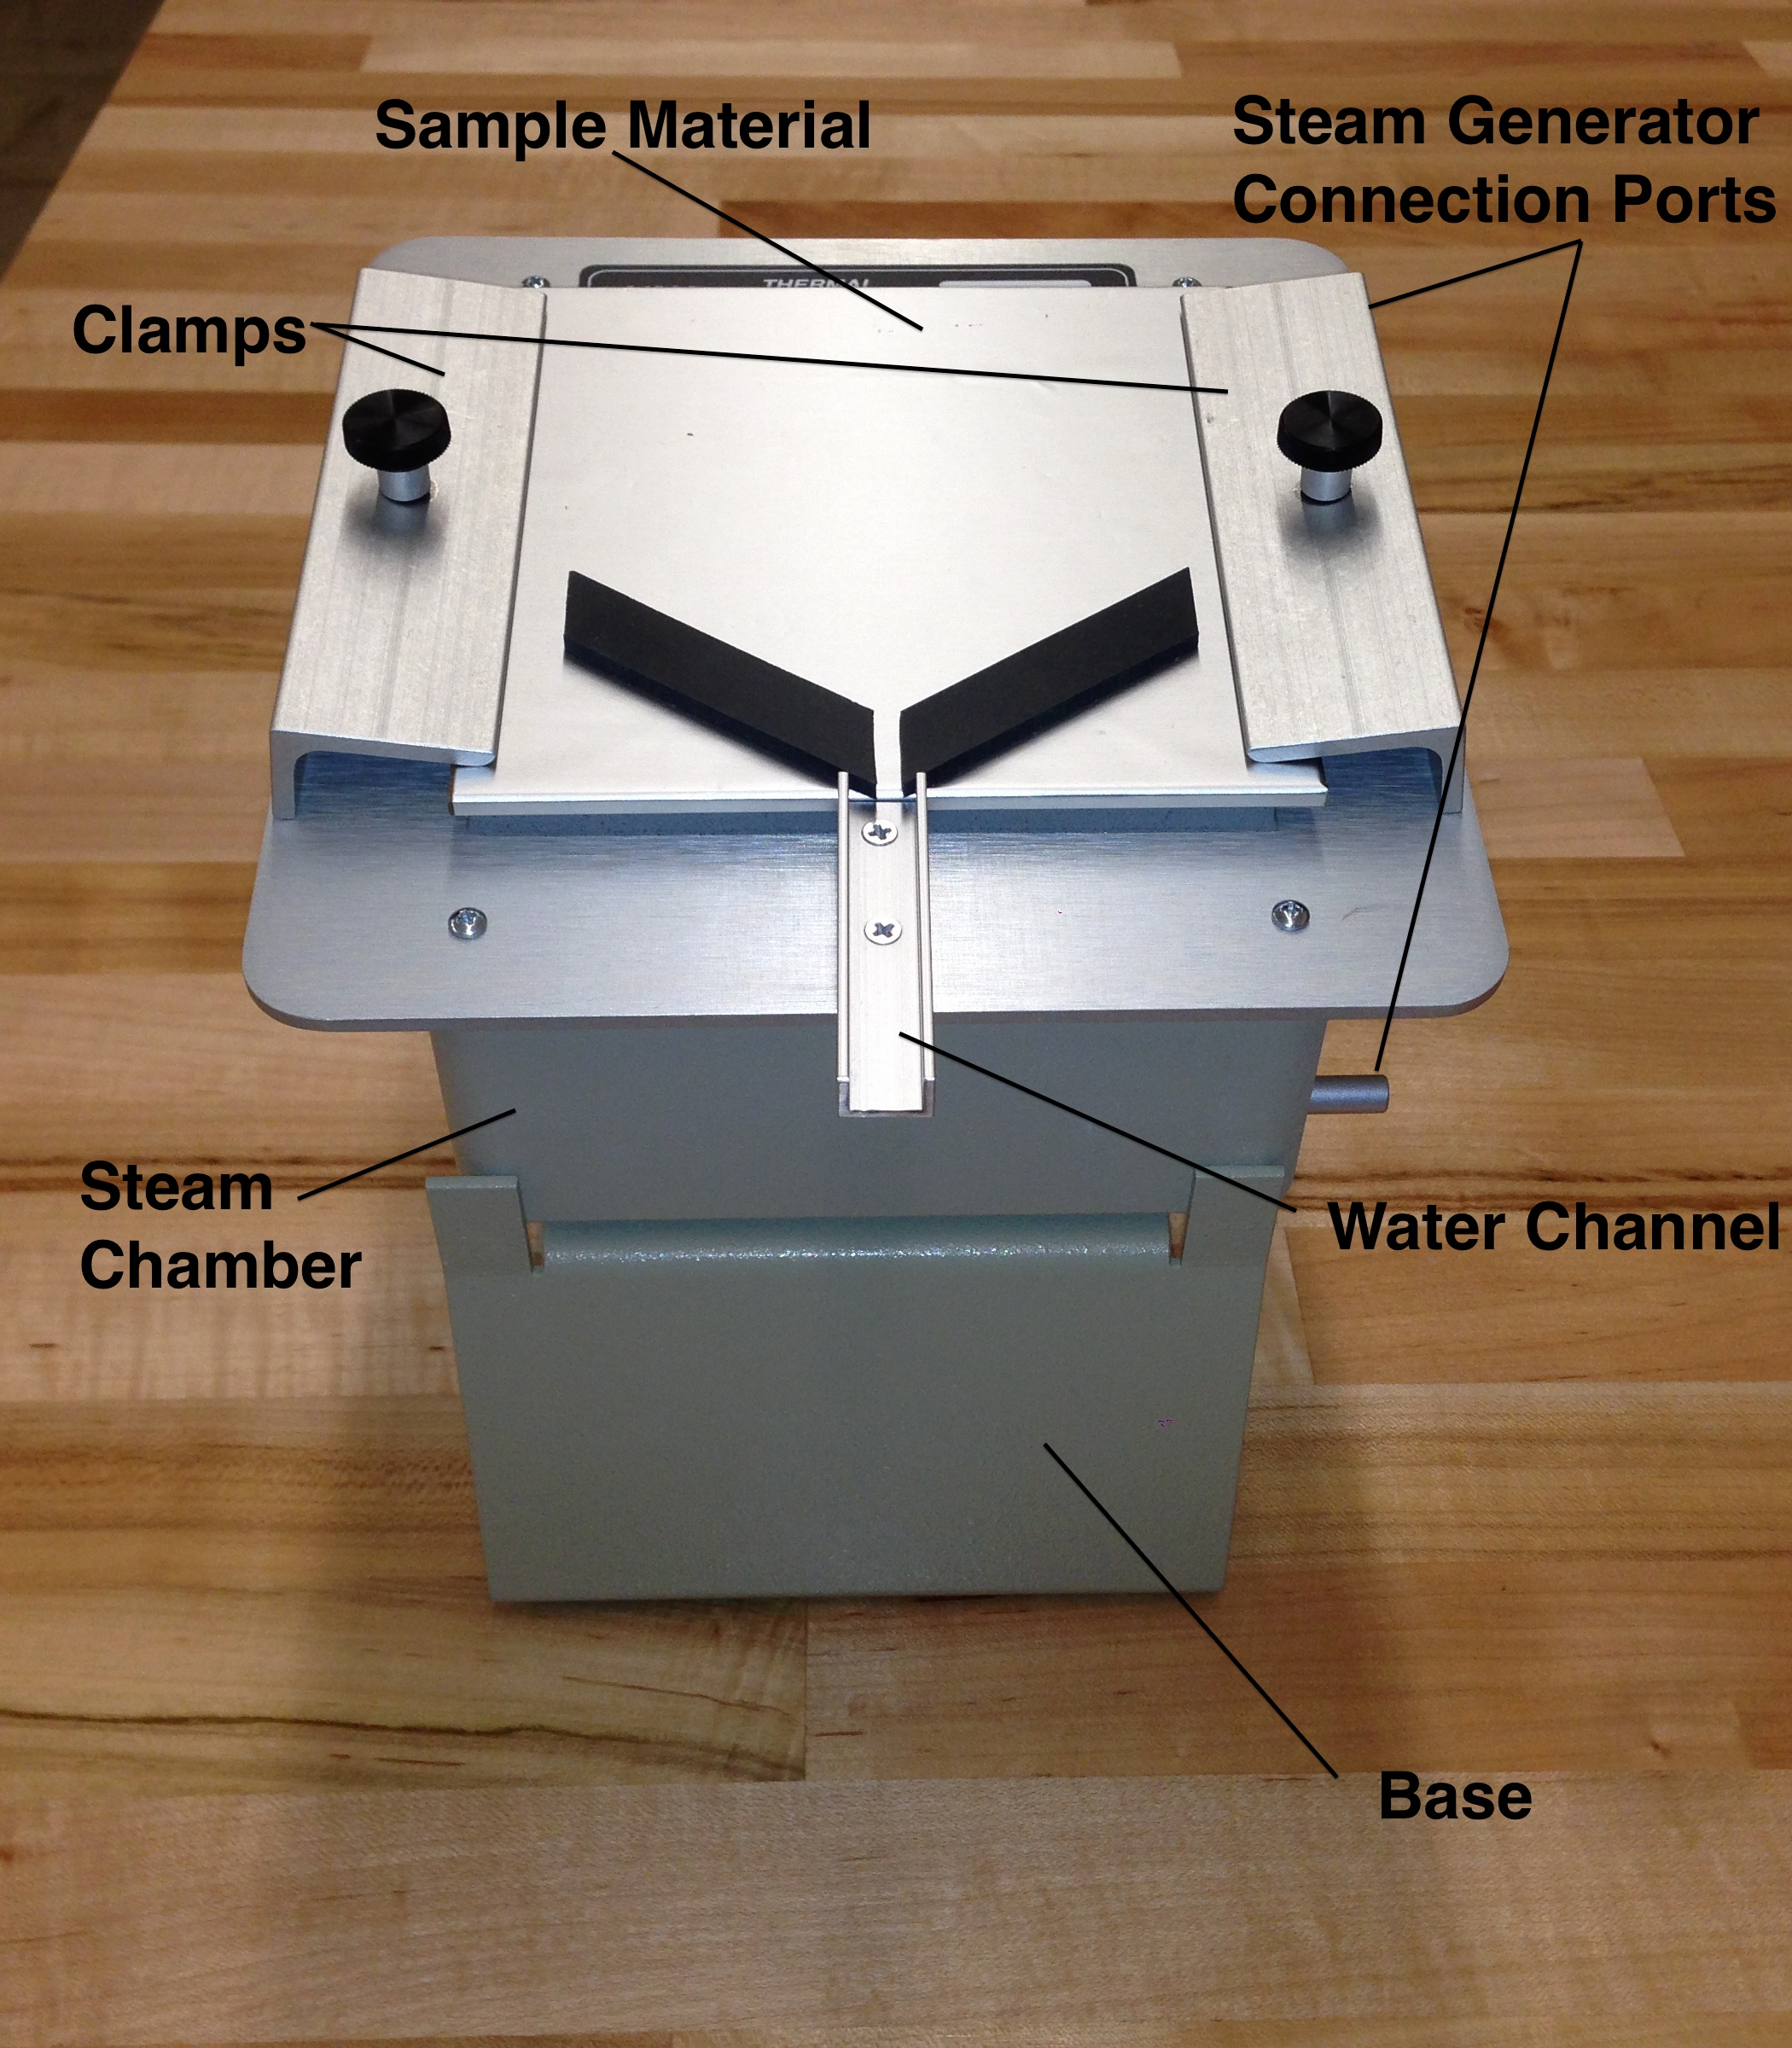
\includegraphics[width=\textwidth]{./Exp10/pic/condapppic.jpeg}
		\caption{Conductivity Apparatus}
		\label{condexp1}
	\end{subfigure}
\begin{subfigure}{0.48\textwidth}
	\centering
	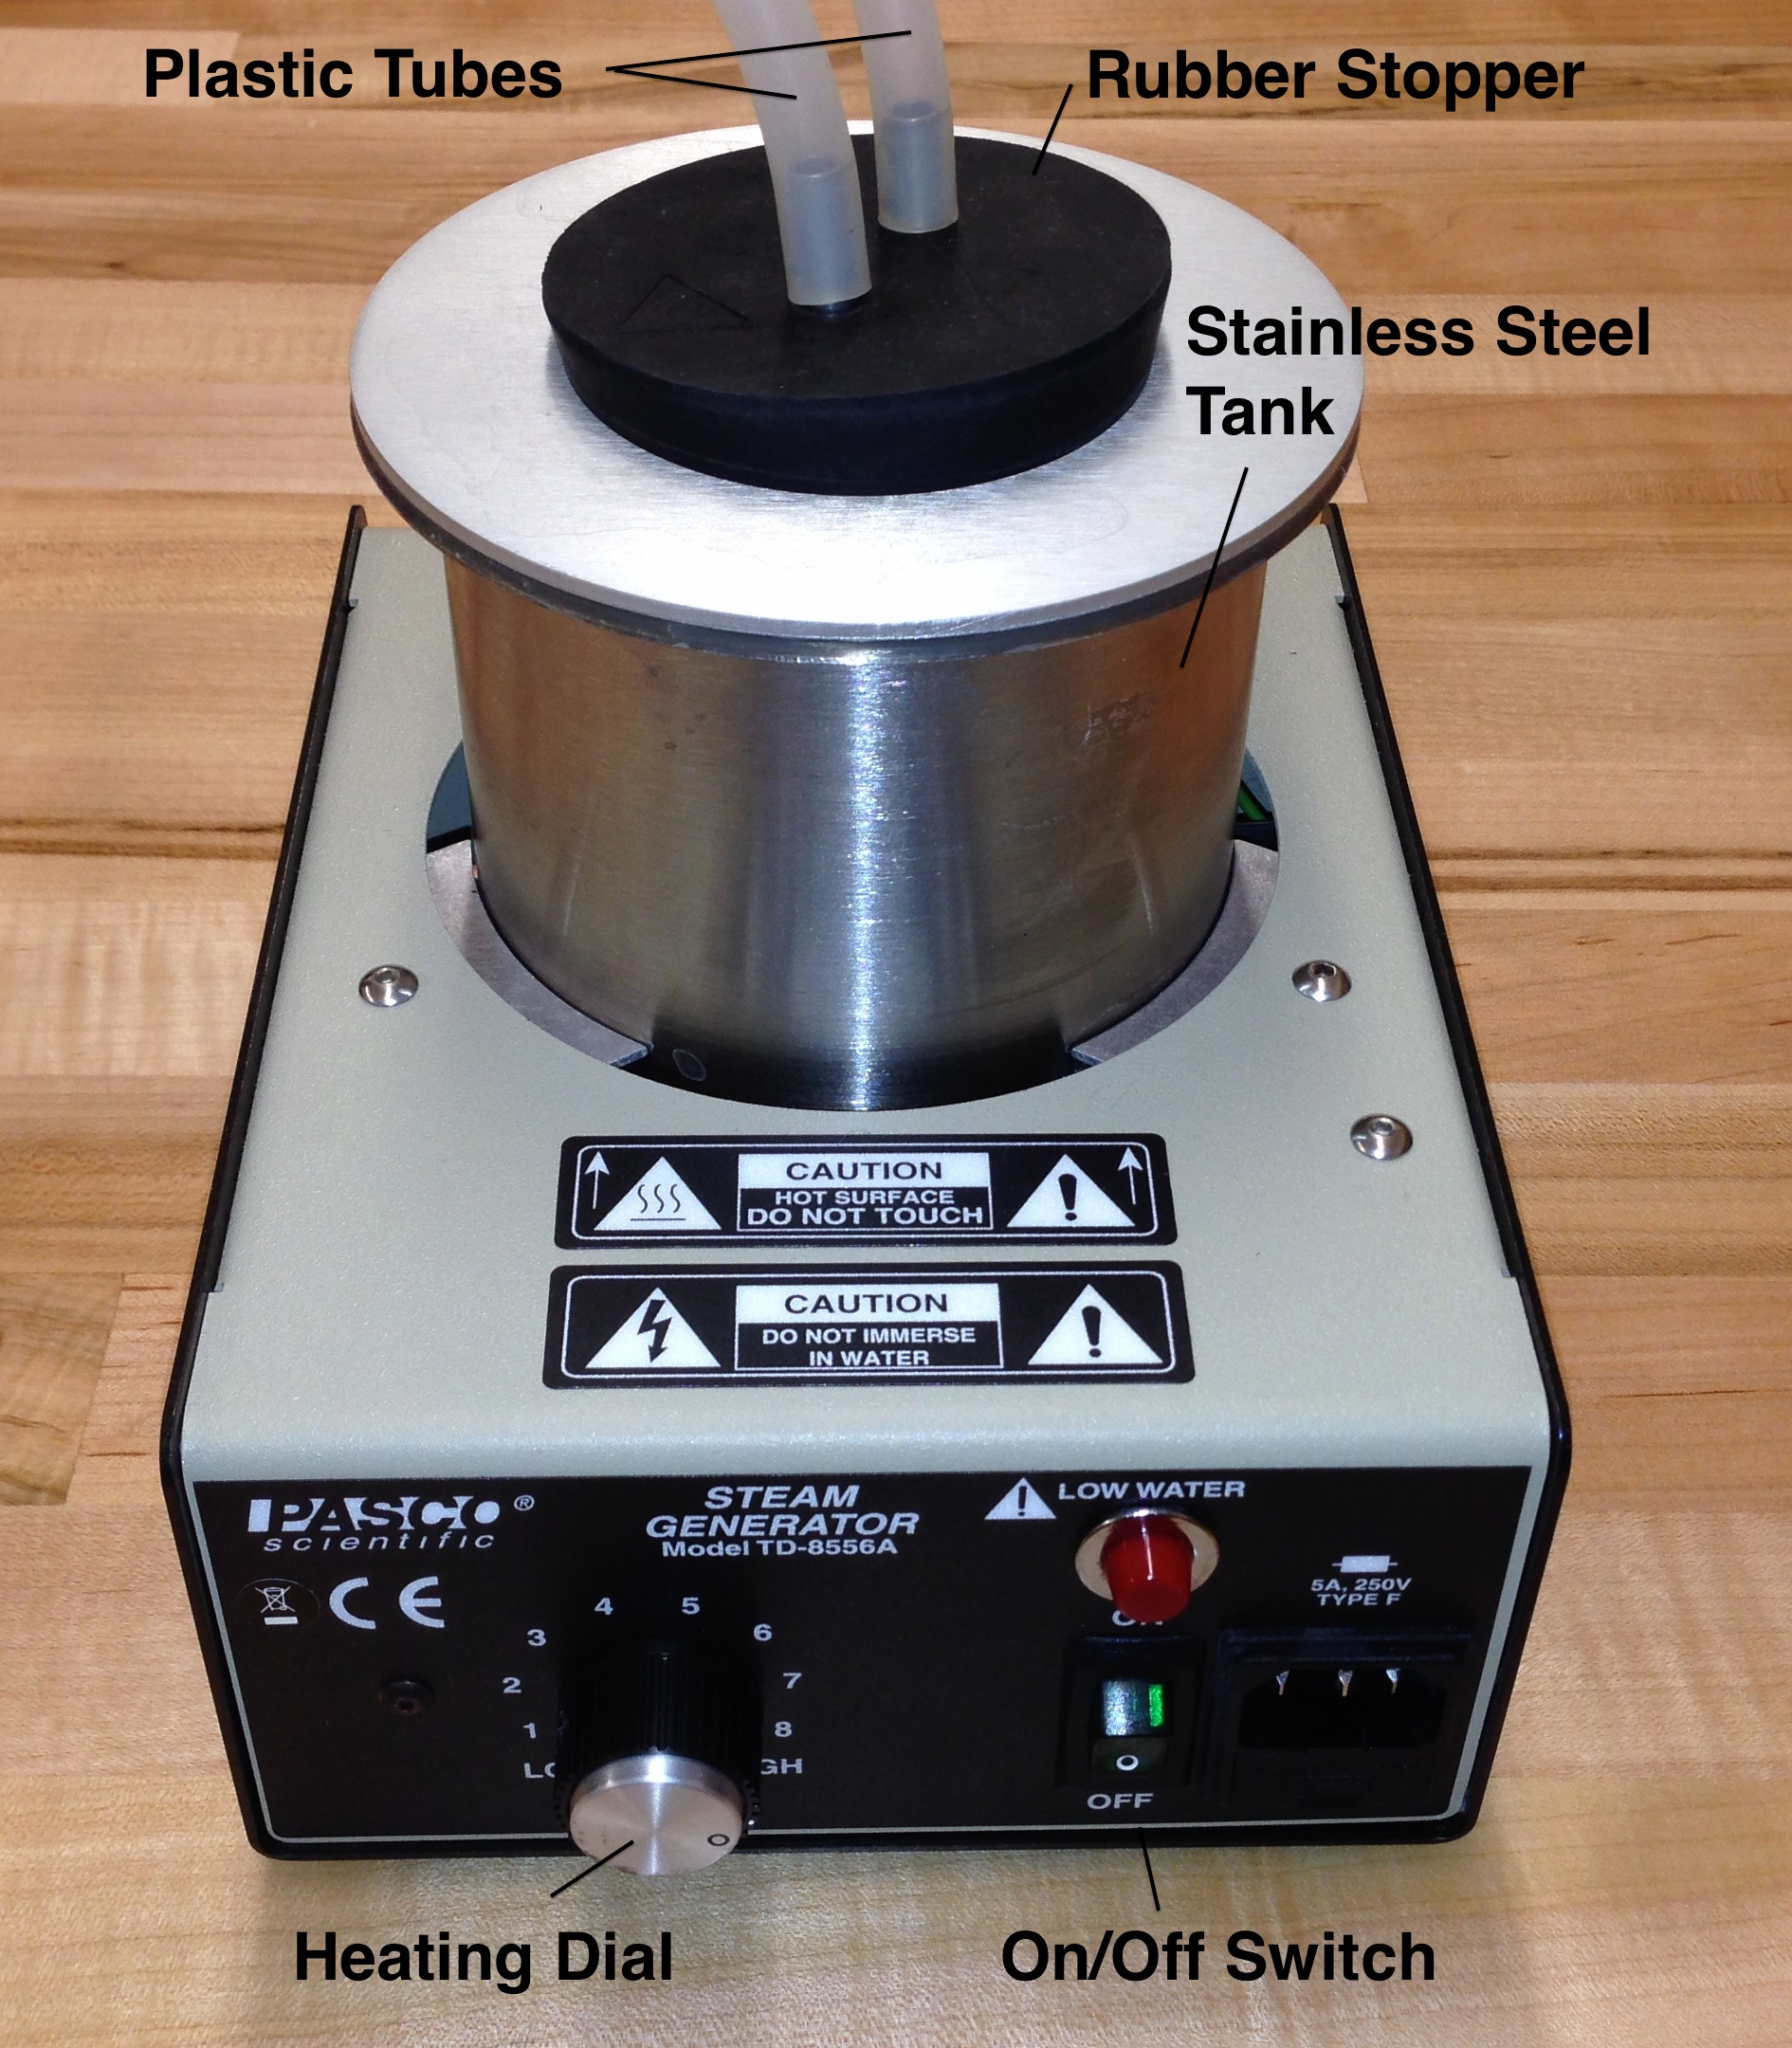
\includegraphics[width=\textwidth]{./Exp10/pic/steamchamberpic.jpeg}
		\caption{Steam Generator}
		\label{condexp2}
\end{subfigure}
\caption{Pictures of the equipment for the thermal conductivity experiment.}
\label{condexp}
\end{figure}

\begin{enumerate}
	\item Begin by ensuring the stainless steel tank of the Steam Generator is 1/2-3/4 full (note that two groups will be sharing a single Steam Generator).  This can be done by lifting the rubber stopper to check the water content - if it is too empty, use a provided cup to add water; if it is too full, use the turkey baster to remove some.  Set the dial to ``HIGH" and power switch to ``ON".  The plastic tubes should NOT yet be connected to the two ports on the rubber stopper or the Steam Chamber on the Thermal Conductivity Apparatus.  \textbf{CAUTION: The stainless steel tank becomes HOT when the unit is on.}
	\item Select any one of the five material samples and using the digital caliper measure its thickness $h$.  Slide it under the clamps on the Thermal Conductivity Apparatus as shown in Figure \ref{condexp1} such that it is pressed tightly against the water channel to prevent leakage.  Tighten the thumbscrews to lock it in place.
	\item Take the block of ice in the cup and run it under gentle water for 5-10 seconds.  The water does not need to be hot.  You should hear the ice crack and loosen.  Take it out of the cup and place it on the first material sample.  Put a paper cup beneath the open end of the water channel to collect water that is melted.
	\item Because the surface of the ice is likely below $273$ K (it should be at the same temperature to which the freezer was set), we will let this sit here for a couple minutes before we begin taking data.  During this time, it is recommended you begin the next experiment in Section \ref{procideal}.
	\item After several minutes the ice should begin to melt at a constant rate.  Lift the ice and measure the diameter $d_B$ of the surface that is touching the sample material.
	\item Take a second paper cup, measure its mass, and replace the first paper cup under the water channel with this one, so that it catches the melted ice.  Begin your timer.  You can empty the first paper cup.
	\item Collect the melting ice for a time $t_{0}$ (suggested 5-10 minutes, or when you feel the cup has accumulated sufficient water) and remove it (you should replace it with the first cup to catch continued water drainage).
	\item Attach the ends of the shorter plastic tube to one port on the Steam Generator, which by now should be producing steam, and the upper port on the side of the Steam Chamber.  Connect the longer tube to the lower port and place the open end into the white plastic pail below the bench that will capture water from steam cooled inside the Steam Chamber.  Let the steam run for a few minutes so the sample material can obtain a steady heat flow.  \textbf{CAUTION: The rubber tubes become HOT when unit is on.  Wear provided gloves when handling.}
	\item Measure the new mass of the second paper cup and subtract from it your empty cup mass measurement to get the mass of the melted water $m_{0}$.  You can then empty the cup.
	\item After several minutes when the heat flow through the sample material appears to be constant, replace the first cup with another empty paper cup and repeat Steps 6, 7, and 9, only now recording $t_{1}$ and $m_{1}$ - the time and mass under these new conditions.  Note: the mass of the ``empty" cup may not be the same in both runs - there may be residual water from the first measurement that adheres to the cup and thus has a slight adjustment on its original mass.
	\item Finally, lift the remaining ice block and re-measure the diameter of the surface touching the sample material.  Record this as $d_A$.
	\item \textbf{Data and Calculations.}  This should serve as a walkthrough for finding $\kappa$ via your measurements and Equation \ref{eq:thermcond}.  Be sure to carry your uncertainty from your measurements through your calculations.  It is recommended you copy and complete Table \ref{vchart}.
	\begin{table}
	\begin{center}
	\begin{tabular}{| c | c| c | c | c | c | c | c || c | c | c | c | c |}
	\hline
	Material & $h$ & $d_B$ & $d_A$& $m_{0}$ & $t_{0}$ & $m_{1}$ & $t_{1}$ & $d_\text{ave}$ & $A$ & $r_{0}$ & $r_{1}$ & $r$ \\
	\hline
	& & & & & & & & & & & &   \\
	\hline
	\end{tabular}
	\end{center}
	\vspace{-0.5 cm}
	\caption{Suggested table for lab report.}
	\label{vchart}
	\end{table}
	\begin{enumerate}
		\item Because the ice is surrounded by air at room temperature, there is a small contribution of ice melt that is not caused by thermal conductivity from the steam.  Thus, $r_{1} \equiv m_{1}/t_{1}$ is the rate of melting due to the thermal conductivity of the sample material plus that of the room temperature air encompassing the remainder of the ice block.  We want to subtract off $r_{0} \equiv m_{0}/t_{0}$ - which corresponds to the rate of ice melt due solely to the heat from the temperature of the room.  The total rate, $r = r_{1} - r_{0}$ should give us the amount of mass melted per unit time caused specifically by the sample material's thermal conduction.
		\item Using Equation \ref{eq:latent} we find $Q/t = mL/t = rL$ (the amount of heat absorbed by the ice per unit time) where $L = 334,000$ J/kg for the ice/water phase transition.
		\item Another consequence of the room melting the exterior of the ice block is there may be a slow decrease in the area of contact of the ice/sample material barrier.  It is likely then you found $d_A < d_B$.  To remedy this we can compute the average diameter $d_\text{ave}$, and using these estimate the average area $A =\pi \left ( \frac{d_\text{ave}}{2}\right )^2$.
		\item Lastly, be sure to use $T_{\rm hot}$ and $T_{\rm cold}$ in Kelvin or Celsius (the difference between two temperatures in both these systems is the same).
\item Calculate the thermal conductivity $\kappa$ with error for your sample material. You can calculate the error in thermal conductivity by propagating uncertainties in measured lengths $d_\text{ave}$ and $h$, masses $m_0$ and $m_1$, and times $t_0$ and $t_1$.
\item  How does your thermal conductivity constant compare to its accepted value in Table \ref{kvalues}?
\item  Discuss the largest sources of error that may have contributed to an incorrect thermal conductivity constant. Do they explain why your result might be larger or smaller than expected?


	\end{enumerate}
	\begin{table}
	\begin{center}
	\begin{tabular}{| c | c |}
	\hline
	Material & $\kappa$ (Watt/m$\cdot$K) \\
	\hline
	Masonite & 0.047 \\
	Wood (Pine) & 0.11-0.14 \\
	Lexan & 0.19 \\
	Sheet Rock & 0.43 \\
	Glass & 0.72-0.86 \\
	\hline
	\end{tabular}
	\end{center}
	\vspace{-0.5 cm}
	\caption{Accepted values for the thermal conductivity $\kappa$ for each of the provided sample materials.}
	\label{kvalues}
	\end{table}
\end{enumerate}

\newpage


\subsection{Ideal Gas Law}
\label{procideal}
In this experiment we will verify the relation between pressure, volume, and temperature for an ideal gas.  Be sure to reference the Ideal Gas Apparatus setup in Figure \ref{idealapp} for the following steps.

\begin{figure}
	\centering
	\begin{subfigure}{0.48\textwidth}
		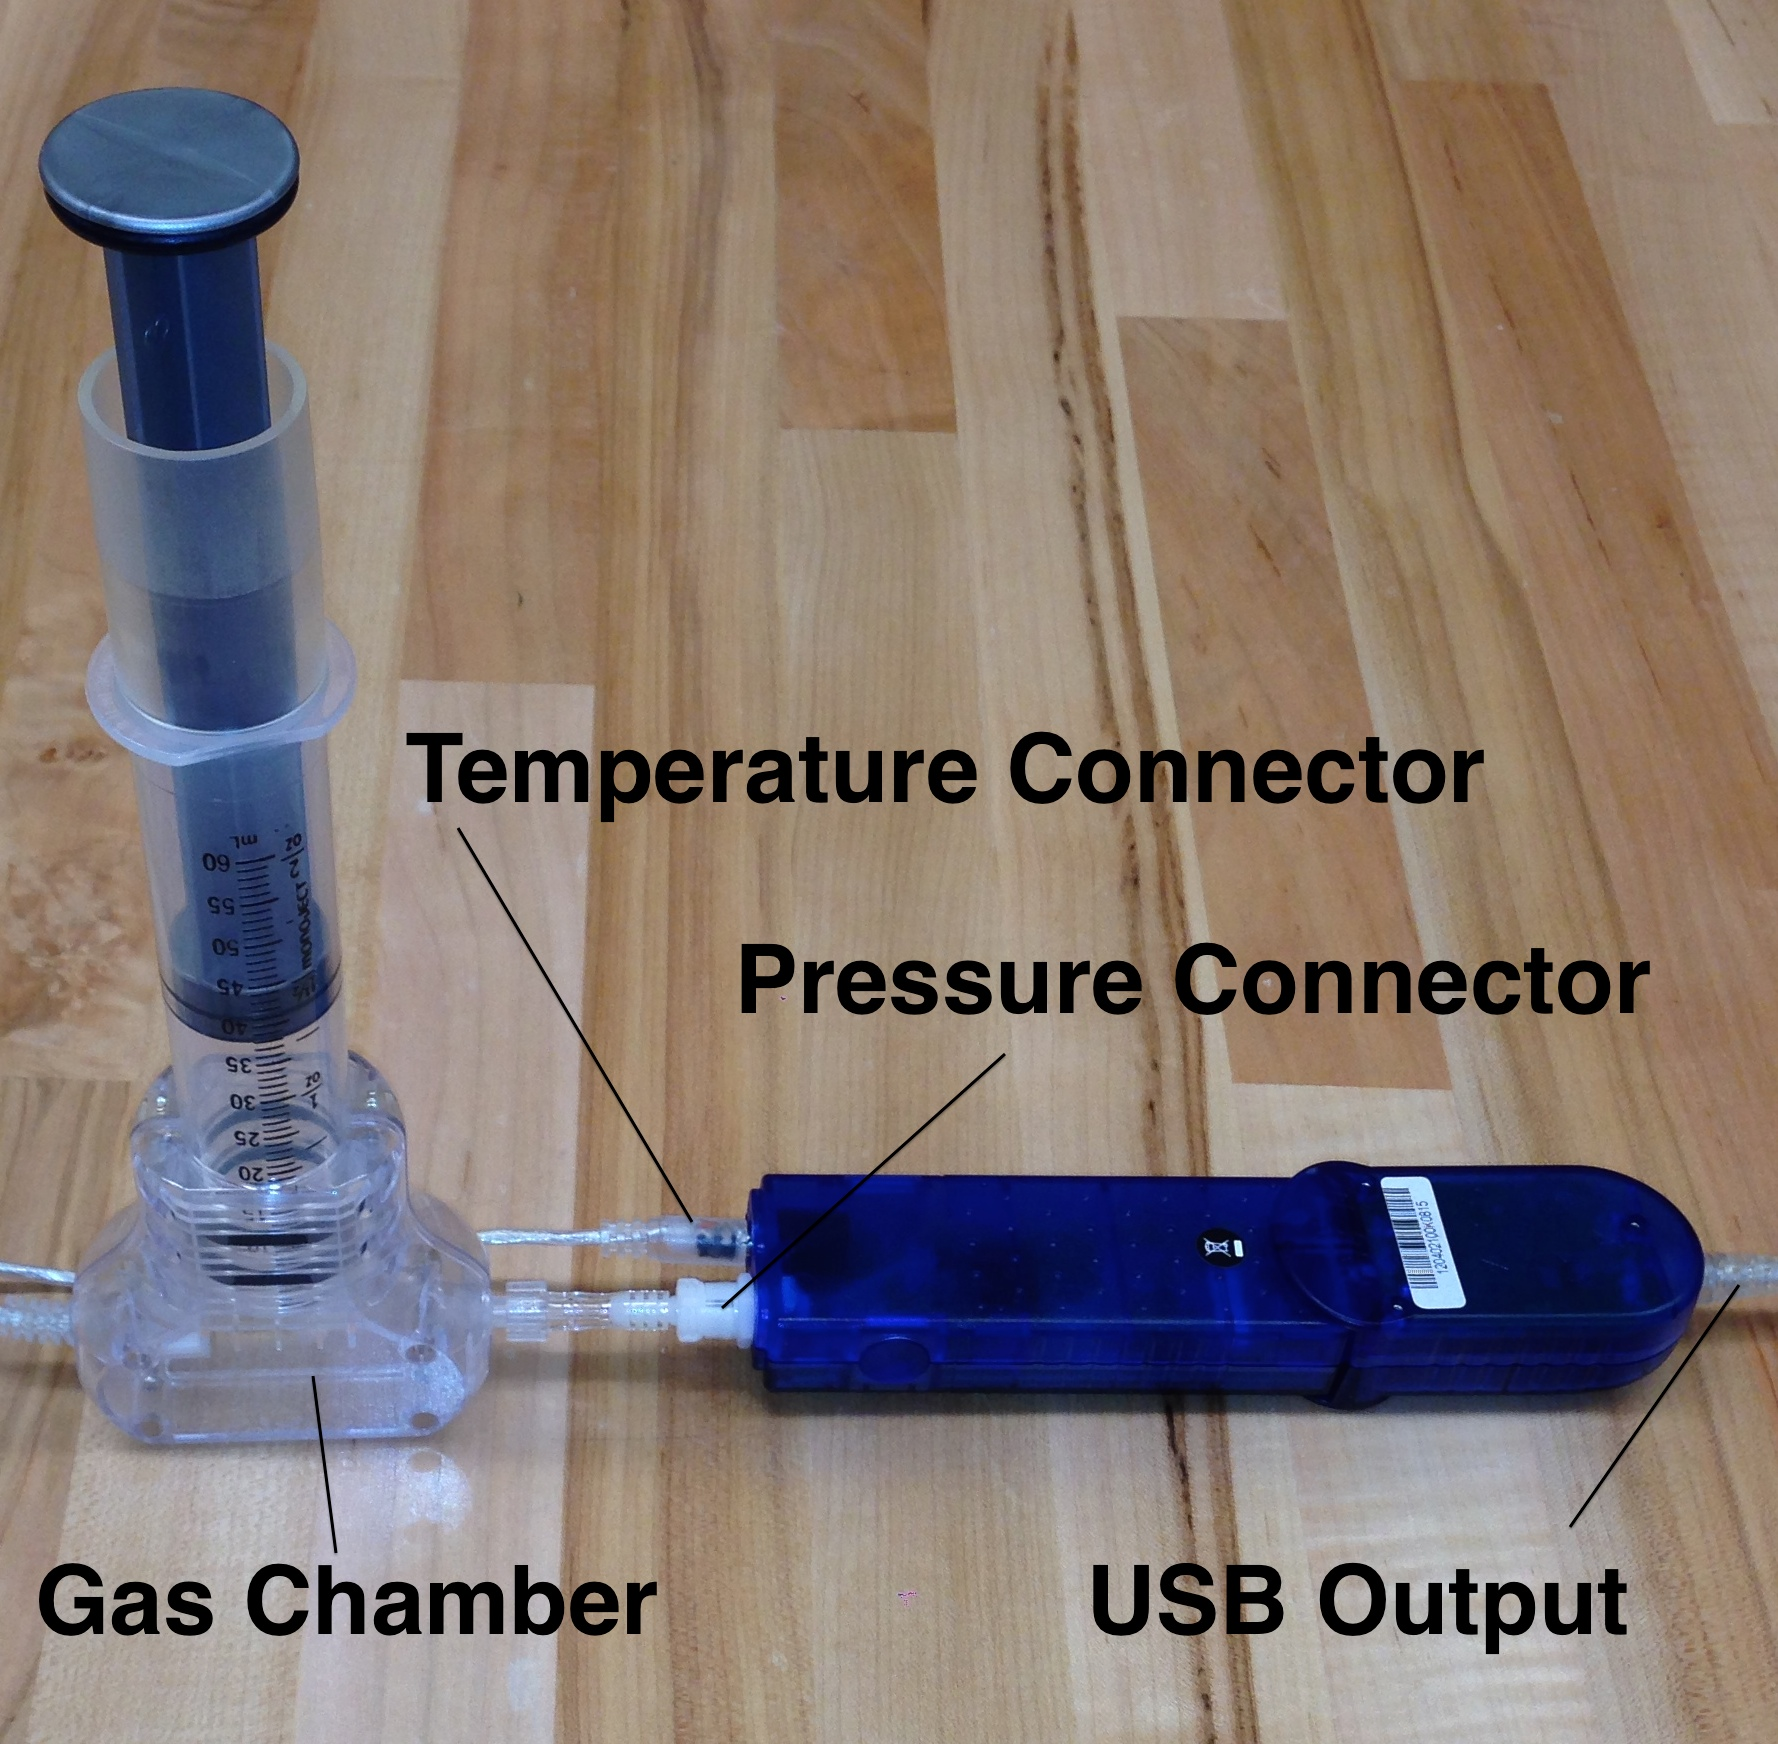
\includegraphics[width=\textwidth]{./Exp10/pic/idealgaspic.jpeg}
	\end{subfigure}
\begin{subfigure}{0.48\textwidth}
	\centering
	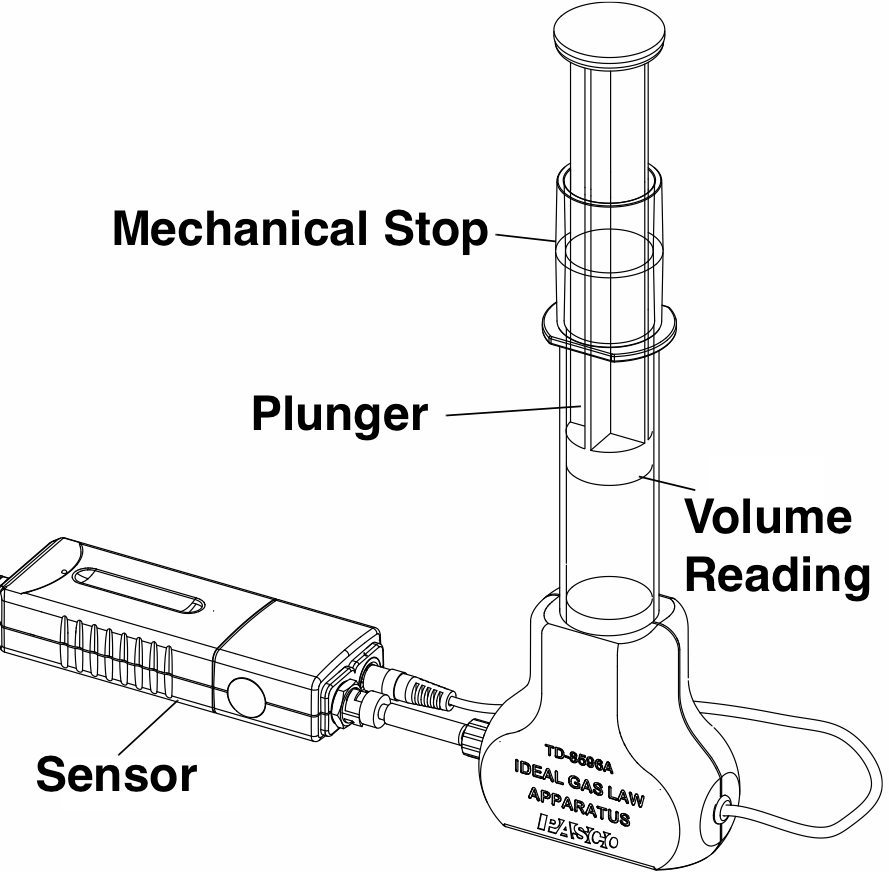
\includegraphics[width=\textwidth]{./Exp10/pic/idealgasdiag}
\end{subfigure}
\caption{Picture and diagram of the Ideal Gas Law Apparatus.}
\label{idealapp}
\end{figure}

\begin{enumerate}
	\item With the pressure connector unplugged from the sensor (see Figure \ref{pdisc}), push the plunger all the way in until it hits the mechanical stop and bottoms out.  Record this volume as $V_{1}$; it should be around $20$ cc.
	\item Lift the plunger until the volume of the plunger is at some new value around $40$ cc.  Record this as $V_{2}$.  Attach the pressure connector and verify the temperature connector is also plugged in.
	\item Ensure the USB output is connected to the computer.  Open the DataStudio file ``Ideal Gas Law" located on the desktop.  You should see graphs and a chart to record pressure and temperature as a function of time.
	\item Click \textbf{Start}.  The program should begin taking data.  Holding the base of the syringe flat against the table, fully and quickly compress the plunger such that it again bottoms out.  Hold it in this position until the temperature and pressure have stabilized and stopped changing.  This should take approximately 30-45 seconds.  Note this is an isochoric process, as your hand preventing the plunger from moving keeps the volume constant while $P$ and $T$ change.
	\begin{figure}
		\centering
		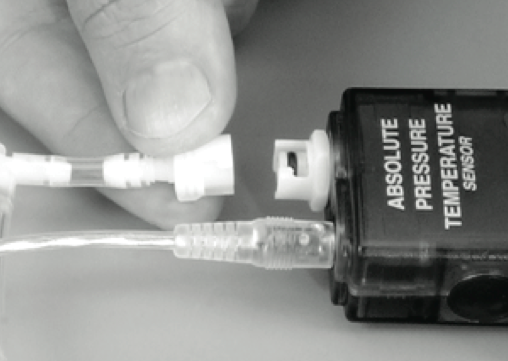
\includegraphics[width=0.5\textwidth]{./Exp10/pic/pressuregaugepic}
		\caption{Disconnecting the pressure connector allows one to change the volume of the gas chamber without affecting the pressure.}
		\label{pdisc}
	\end{figure}

	\item Release the plunger and allow it to expand back out on its own (it may not return to $V_{2}$).  Again, permit the pressure and temperature to approach at some equilibrium values.  Click \textbf{Stop}.
	\item \textbf{Data and Calculations - Constant $T$}
	\begin{enumerate}
		\item Highlight a section of the pressure graph early in the run before the compression (around $V_{2}$).  You should see the corresponding (roughly constant) values show in the data table - call this $P_{2}$.
		\item Highlight a section of the pressure graph just before you released the piston (at $V_{1}$).  Again, use the roughly constant values in the data table to determine the pressure $P_{1}$.
		\item You should notice that at both these values, the temperatures were approximately the same.  Why is this?  How does this relate to Section \ref{proctherm}?  Because the gas chamber does not allow any air molecules to escape (i.e. $N$ is constant) we find
		\begin{equation}
			P_{1}V_{1} = NkT = P_{2}V_{2} \textrm{\, \, or \, \,} \frac{V_{1}}{V_{2}} = \frac{P_{2}}{P_{1}} \textrm{.}
		\end{equation}
		Are these equal?  How much do they differ by?  It turns out both $V$ are off by a common factor; the volume reader does not account for the small region of tubing that connects the gas chamber to the sensor.  If we now factor in this small quantity $V_{0}$ we can write
		\begin{equation}
			\frac{V_{1}+V_{0}}{V_{2}+V_{0}} = \frac{V^{\prime}_{1}}{V^{\prime}_{2}} = \frac{P_{2}}{P_{1}} {\rm .}
		\end{equation}
		where we define the true volumes $V^{\prime}_{1}=V_{1}+V_{0}$ and $V^{\prime}_{2}=V_{2}+V_{0}$.  Solve for $V_{0}$.
		\item Why doesn't the plunger return to its original volume $V_{2}$ after an extended period of time?  (Hint: consider the force that the pressure from the gas exerts upward on the plunger, and any forces that may oppose it.)
	\end{enumerate}
	\item \textbf{Data and Calculations - Varying $T$}
	\begin{enumerate}
		\item Highlight a region on the temperature graph at the beginning of the run before the compression (it does not matter if it is the same point as above).  Record the pressure $P_{3}$ and temperature $T_{3}$.
		\item Highlight a region on the temperature graph where $T$ is a maximum.  Record the pressure $P_{4}$ and peak temperature $T_{4}$.  Note: it is important you choose a set of points at the same time where $T$ is a maximum, even if this does not correspond to $P$ being a maximum.
		\item Calculate
		\begin{equation}
			\frac{P_{3}V^{\prime}_{2}}{T_{3}} \textrm{\, \, and \, \,} \frac{P_{4}V^{\prime}_{1}}{T_{4}}
		\end{equation}
		and determine if they are equivalent.  (Remember to include $V_{0}$ in your volume measurements as with last section.)  Note that here we are assuming the temperature is a maximum when the plunger is fully compressed.  Using Equation \ref{eq:firstlaw} and Section \ref{procadiab}, explain why quickly compressing the plunger was essential to this result.  Related to this, qualitatively explain why there was a dramatic increase in $P$ (much more than the inverse ratio of the volumes).
		\item When the plunger is finally released, what initially happens to the temperature?  Why?
	\end{enumerate}
	\item Exit out of DataStudio.  Do not save your data.
\end{enumerate}

\subsection{Adiabatic Compression (Demo)}
\label{procadiab}
This experiment will be a demonstration of using adiabatic compression to ignite a small piece of tissue paper.  This only needs to be done once in front of the entire class and you do not have to take data - however, you should be able to explain your observations with the assistance of Section \ref{idealtheory}.

\begin{figure}
	\centering
	\begin{subfigure}{0.48\textwidth}
		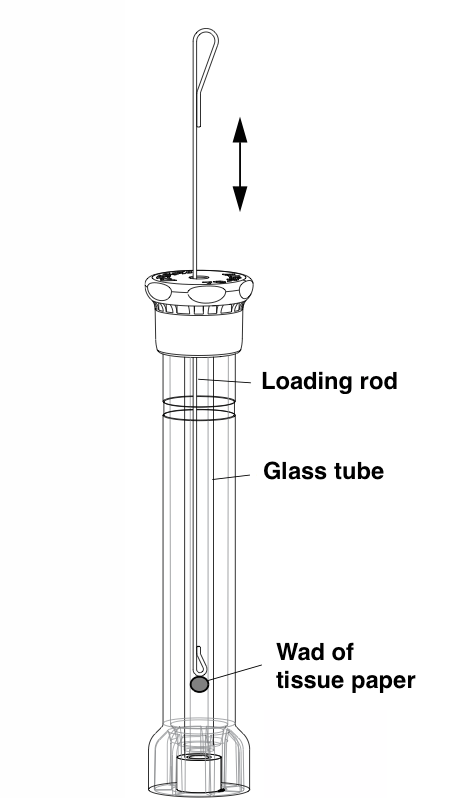
\includegraphics[width=0.9\linewidth]{./Exp10/pic/adiabsetup}
		\caption{Setup}
	\end{subfigure}
\begin{subfigure}{0.48\textwidth}
	\centering
	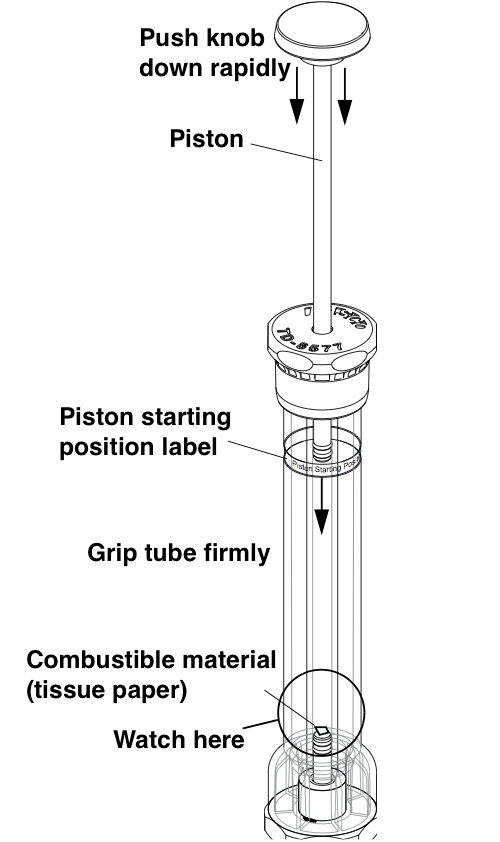
\includegraphics[width=0.9\linewidth]{./Exp10/pic/adiabignite}
	\caption{Compression Igniter}
\end{subfigure}
\caption{Diagram of how to setup and use the Compression Igniter.}
\label{adiabapp}
\end{figure}

\begin{enumerate}
	\item Remove the piston from the Compression Ignitor and with the loading rod, push a small ($\sim 1 \, {\rm cm}^{2}$) wad of tissue paper into the lower part of the glass tube.  Be careful to not crumble the tissue paper much, so that its surface is maximized.
	\item Carefully remove the loading rod and reinsert the piston.  Place the base of the Compression Ignitor on the surface of the table and securely hold the tube with one hand.  It is recommended you dim or turn off the lights in the room.
	\item With the palm of your hand, quickly slap down on the knob of the piston so it rapidly goes down the cylinder.  You should see the paper ignite.  Note: it requires a fair amount of force to light the tissue.  Consequently, this only needs to be done once per class, by either the TA or a student in the lab section.  If the paper does not initially ignite, try again.  If after several attempts it has still not ignited, try replacing the wad of paper with a smaller sample.
	\item \textbf{Questions}
	\begin{enumerate}
		\item What happens to the air as the plunger is compressed?  How does this lead to the paper lighting on fire?
		\item Why is compressing the plunger quickly essential to this experiment?  How would the results change if you did so slowly?  Why?
	\end{enumerate}
\end{enumerate}
